% ICCV 2025 Paper Template

\documentclass[10pt,twocolumn,letterpaper]{article}
%%%%%%%%% PAPER TYPE  - PLEASE UPDATE FOR FINAL VERSION
\usepackage{iccv}              % To produce the CAMERA-READY version
% \usepackage[review]{iccv}      % To produce the REVIEW version
\usepackage{multirow}
\usepackage{ulem} 
\usepackage{amsmath,amssymb,bm}
% \usepackage[pagenumbers]{iccv} % To force page numbers, e.g. for an arXiv version
% Import additional packages in the preamble file, before hyperref
% %
% --- inline annotations
%
\newcommand{\red}[1]{{\color{red}#1}}
\newcommand{\todo}[1]{{\color{red}#1}}
\newcommand{\TODO}[1]{\textbf{\color{red}[TODO: #1]}}
% --- disable by uncommenting  
% \renewcommand{\TODO}[1]{}
% \renewcommand{\todo}[1]{#1}


% It is strongly recommended to use hyperref, especially for the review version.
% hyperref with option pagebackref eases the reviewers' job.
% Please disable hyperref *only* if you encounter grave issues, 
% e.g. with the file validation for the camera-ready version.
%
% If you comment hyperref and then uncomment it, you should delete *.aux before re-running LaTeX.
% (Or just hit 'q' on the first LaTeX run, let it finish, and you should be clear).
\definecolor{iccvblue}{rgb}{0.21,0.49,0.74}
\usepackage[pagebackref,breaklinks,colorlinks,allcolors=iccvblue]{hyperref}

\pdfobjcompresslevel=0

%%%%%%%%% PAPER ID  - PLEASE UPDATE
\def\paperID{4687} % *** Enter the Paper ID here
\def\confName{ICCV}
\def\confYear{2025}

\newcommand{\model}{VoRA}
\newcommand{\mllm}{Multimodal LLM}
\newcommand{\mono}{Multimodal Native LLM}


%%%%%%%%% TITLE - PLEASE UPDATE
\title{Vision as LoRA}

%%%%%%%%% AUTHORS - PLEASE UPDATE
\author{%
  Han Wang$^{1}$ \hspace{1.5cm} % 调整间距
  Yongjie Ye$^{1}$ \hspace{1.5cm}
  Bingru Li$^{2}$ \hspace{1.5cm}
  Yuxiang Nie$^{1}$ \\ 
  Jinghui Lu$^{1}$ \hspace{1.2cm}
  Jingqun Tang$^{1}$ \hspace{1.2cm}
  Yanjie Wang$^{1}$ \hspace{1.2cm}
  Can Huang$^{1}$ 
  \\
  $^1$ByteDance Inc. \   \ $^2$University of Birmingham
}


\begin{document}
\maketitle
\begin{abstract}
Fine-tuning provides an effective means to specialize pre-trained models for various downstream tasks. However, fine-tuning often incurs high memory overhead, especially for large transformer-based models, such as LLMs. While existing methods may reduce certain parts of the memory required for fine-tuning, they still require caching all intermediate activations computed in the forward pass to update weights during the backward pass. In~this work, we develop \method, a method to reduce memory usage,  specifically the memory to store intermediate activations, in the fine-tuning of transformer-based models. During the backward pass, \method approximates the gradient computation by backpropagating through just a subset of input tokens. Thus, with \method, only a subset of intermediate activations are cached during the forward pass. Also, \method can be easily combined with existing methods like LoRA, further reducing the memory cost. We evaluate our approach on pre-trained transformer models with up to billions of parameters, considering the performance on multiple downstream tasks such as text classification and question answering in a few-shot learning setup. Overall, \method achieves performance on par with full fine-tuning or representative memory-efficient fine-tuning methods,  while greatly reducing the memory footprint, especially when combined with other methods with complementary memory reduction mechanisms. We hope that our approach will facilitate the fine-tuning of large transformers,  in specializing them for specific domains or co-training them with other neural components from a larger system. Our code is available at \githubURL.
\blfootnote{\textbf{*} Equal contribution}
\end{abstract}
    
\section{Introduction}
\label{sec:intro}

\begin{figure*}[t!]
    \centering
    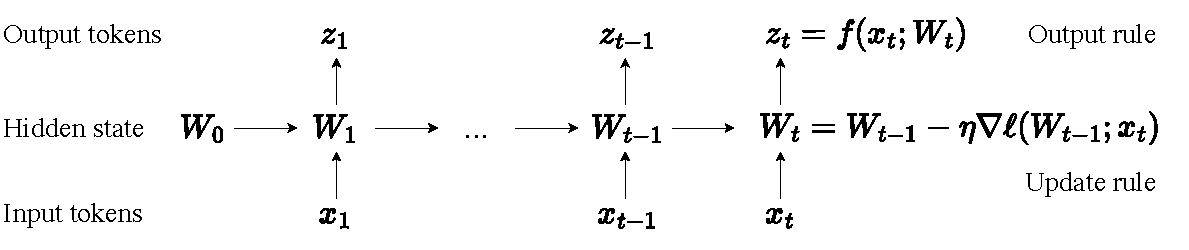
\includegraphics[width=0.8\textwidth]{figs/simple_teaser.pdf}
    \caption{All RNN layers can be expressed as a hidden state that transitions according to an update rule.
    The key idea in \cite{sun2024ttt} is to make the hidden state itself a model $f$ with weights $W$, and the update rule a gradient step on the self-supervised loss $\ell$.
    Therefore, updating the hidden state on a test sequence is equivalent to training the model $f$ at test time. 
    This process, known as Test-Time Training (TTT), is programmed into TTT layers. 
    Figure and caption taken from \cite{sun2024ttt}.
    }
    \label{fig:ttt-layer}
\end{figure*}

Despite the remarkable progress in visual and physical realism, state-of-the-art video Transformers are still generating mostly short clips of single scenes without complex stories.
At the time of writing (March 2025), the maximum length of public APIs for video generation is 20 seconds for Sora (OpenAI), 16 seconds for MovieGen (Meta), 10 for Ray~2 (Luma), and 8 for Veo~2 (Google).
None of these APIs can autonomously generate complex multi-scene stories.

A fundamental challenge behind these technical limitations is long context, because the cost of self-attention layers in Transformers increases quadratically with context length.
This challenge is especially acute for video generation with dynamic motion, whose context cannot be easily compressed by a tokenizer.
Using a standard tokenizer, each of our one-minute videos requires over 300k tokens in context. 
With self-attention, generating a one-minute video would have taken $11\times$ longer than generating 20 videos of 3 seconds each, and training would have taken $12\times$ longer.

To address this challenge, recent work on video generation has investigated RNN layers as an efficient alternative to self-attention, because their cost increases linearly with context length~\cite{wang2024lingenhighresolutionminutelengthtexttovideo}.
Modern RNN layers, especially variants of linear attention~\cite{schmidhuberlinearattn, katharopoulos2020lineartransformers} such as Mamba~\cite{gu2024mamba, dao2024mamba2} and DeltaNet~\cite{schlag2021deltanet, yang2025gateddeltanetworksimproving}, have shown impressive results for natural language tasks.
However, we have yet to see long videos with complex stories or dynamic motion generated by RNNs.
Videos (\href{https://lineargen.github.io/}{link}) in \cite{wang2024lingenhighresolutionminutelengthtexttovideo} are high resolution and one-minute long, but contain only single scenes and slow motion, let alone complex stories.

We believe that these RNN layers generate less complex videos because their hidden states are less expressive.
RNN layers can only store past tokens into a hidden state of fixed size, which is only a matrix for linear attention variants such as Mamba and DeltaNet.
It is inherently challenging to compress hundreds of thousands of vectors into a matrix with only thousands in rank.
As a consequence, these RNN layers struggle to remember the deep relationships between distant tokens.

We experiment with an alternative class of RNN layers whose hidden states themselves can be neural networks. Specifically, we use two-layer MLPs with 2$\times$ more hidden cells and richer nonlinearities than the linear (matrix) hidden states in linear attention variants.
Since the neural network hidden states are updated by training even on test sequences, these new layers are called Test-Time Training (TTT) layers~\cite{sun2024ttt}.

We start from a pre-trained Diffusion Transformer (CogVideo-X 5B \cite{hong2023cogvideo}) that could only generate 3-second short clips at 16 fps (or 6 seconds at 8 fps).
Then, we add TTT layers initialized from scratch and fine-tune this model to generate one-minute videos from text storyboards. 
We limit the self-attention layers to 3-second segments so their cost stays manageable.
With only preliminary systems optimization, our training run takes the equivalent of 50 hours on 256 H100s.

We curate a text-to-video dataset based on $\approx$ 7 hours of \textit{Tom and Jerry} cartoons with human-annotated storyboards.
We intentionally limit our scope to this specific domain for fast research iteration.
As a proof-of-concept, our dataset emphasizes complex, multi-scene, and long-range stories with dynamic motion, where progress is still needed; it has less emphasis on visual and physical realism, where remarkable progress has already been made.
We believe that improvements in long-context capabilities for this specific domain will transfer to general-purpose video generation.

Compared to strong baselines such as Mamba 2~\cite{dao2024mamba2}, Gated DeltaNet~\cite{yang2025gateddeltanetworksimproving}, and sliding-window attention layers, TTT layers generate much more coherent videos that tell complex stories with dynamic motion, leading by 34 Elo points in a human evaluation of 100 videos per method.
For context, GPT-4o scores 29 Elo points over GPT-4 Turbo in LMSys Chatbot Arena~\cite{chiang2024chatbot}.

Sample videos, code and annotations are available at:
\url{https://test-time-training.github.io/video-dit}
\section{Related Works}
\label{sec:related}
\subsection{Encoder-based MLLMs}
The dominant architecture of MLLMs has remained largely unchanged since its inception, comprising three components: a ViT \cite{clip, siglip, aimv2}, an LLM \cite{llama, gpt3, qwen2.5, vicuna}, and a connector to bridge modality gaps. Previous research has focused primarily on connector design, ranging from simple MLP layers \cite{llava, llava1_5, minigpt, minigptv2} to hierarchical feature fusion modules \cite{flamingo, llama3.2} or other complex architectures \cite{elysium, dynamicvlm, internvl, cambrian1}. Despite these innovations, fundamental limitations persist due to their reliance on external vision encoders. First, computational and memory overhead escalates dramatically when applying multiple vision encoders \cite{cambrian1} or scaling to larger ones \cite{cogvlm}. Second, fixed-resolution pre-training of ViTs forces MLLMs to employ workarounds like image tiling \cite{llava1_5, llavaov} or restricted square resolutions \cite{cogvlm, qwen}. Recent attempts \cite{pixtral, qwen2vl, aimv2} to train resolution-agnostic ViTs have remained impractical, in that they adopted massive proprietary data and opaque training procedures. These challenges have spurred interest in encoder-free architectures that could bypass ViTs entirely.
\subsection{Encoder-free MLLMs}
The pioneering work, Fuyu \cite{fuyu}, demonstrated the feasibility of training encoder-free models on interleaved image-text data, though at prohibitive computational costs with limited technical transparency. Subsequent approaches, such as EVE \cite{eve}, reduced the vision encoder parameters to a single Transformer block, aligning its output features with a ViT through distillation while updating all LLM parameters to learn about vision during the main training stage. However, these methods still struggle with conflicts between the LLM’s inherent language abilities and the new modality, i.e., vision. These conflicts arise from the coupled language and vision parameters, which exacerbate unstable training and lead to catastrophic forgetting of the original language abilities.
% Fuyu \cite{fuyu} pioneered such an approach by training on interleaved image-text data. However, this method required substantial computational resources and the detailed technic is unavalable. Subsequent efforts, such as EVE \cite{eve}, explored converting pre-trained LLMs into MLLMs by replacing ViTs with a single transformer block and aligning features via a distillation-like method. This can be understood as reducing the parameters of the vision encoder. During their main stage training, all LLM parameters are updated. Such methods have certain issues, where the modality confliction between a well-pretrained LLM and a new modality that LLM has never seen before remains a severe problem that can easily cause the training unstable, and even we can stablize the training, such method suffer from catastropic forgetting issue.

To overcome these problems, Mono-InternVL \cite{monointernvl} and EVEv2 \cite{evev2} proposed parameter decoupling strategies inspired by the MoE method \cite{moe}, duplicating LLM parameters for vision-specific processing while freezing its original weights. Despite successfully addressing forgetting issues and modality conflicts, these methods suffered from substantial memory overhead by doubling model parameters, compromising architectural simplicity. 
% This tension highlights a critical insight: preserving LLM integrity while integrating vision understanding requires strict parameter decoupling without persistent duplication. 
Our work addresses this by applying LoRA, which encodes vision while maintaining the language abilities of the LLM, and can be merged into the LLM without causing additional memory overhead.
%while maintaining modality alignment.


% \subsection{Encoder-based MLLM}
% The mainstream architecture of MLLMs follows the “Vision-Connector-LLM” framework, consisting of three key components: the vision encoder(s), the connector, and the LLM. Below, we examine these components in detail.
% \\
% \textbf{vision Encoder}
% The vision encoders used in MLLMs are often trained with contrastive learning loss on image-text tasks, such as CLIP. Additionally, there are other vision encoders trained on vision tasks using self-supervised or semi-supervised objectives. These pre-trained vision encoders provide strong prior knowledge in vision, making them widely adopted in MLLMs.
% \\
% \textbf{Connector}
% Due to the misalignment between the semantic spaces of vision encoders and LLMs, a connector is typically required to bridge this gap, which is one of the most distinctive functions of the connector. Its architecture can vary based on its additional functions, such as re-sampling to reduce the number of visual tokens.
% \\
% \textbf{LLM}
% The LLM often serves as the core component of the architecture, consuming the majority of computations and parameters. These models are typically developed by large companies or organizations due to the substantial amounts of data and training costs involved. The open community usually focuses on post-training enhancements or develops MLLMs based on existing LLMs.
% \subsection{\mono}
% We define \mono as utilizing a single Transformer, specifically an LLM, to perform multimodal tasks. This architecture requires only a few parameters to convert the dimensionality of data from other modalities, such as using a patchifier for vision, without the need for additional pre-trained models. The explorations of this kind of architecture emerges quite early, but soon struggles in several problems caused by the big gap between 
\section{Vision as LoRA}
\label{sec:methods}
\begin{figure*}
    \centering
    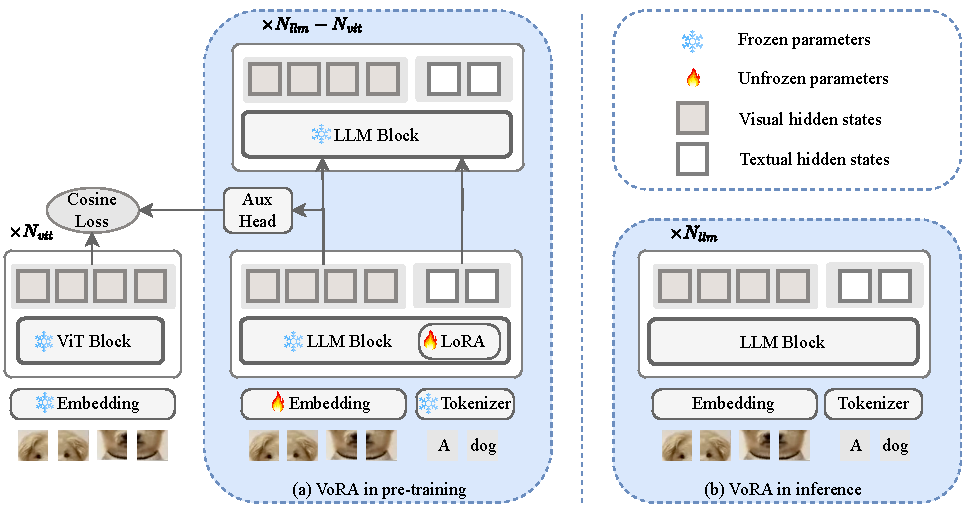
\includegraphics[width=\linewidth]{images/Figure2.pdf}
    \caption{The architecture of \model{}. Figure (a) shows the architecture of \model{} in pre-training: in this stage, \model{} only unfreezes the LoRA layers for vision and the visual embedding layer, i.e., a shallow MLP layer with a positional embedding. Figure (b) shows \model{} in inference: the LoRA layers are merged into the LLM, and thus the only added parameters are a shallow embedding layer (about 6M parameters).}
    \label{fig:architecture}
\end{figure*}
In this section, we introduce three key components of \model{}: vision as LoRA, block-wise distillation, and bi-directional attention masks for vision. 

\subsection{Stabilize training: Vision as LoRA}

As shown in Figure \ref{fig:architecture}(a), we integrate LoRA layers into the LLM to enable vision understanding. During pre-training, images are first converted into vision embeddings using a lightweight embedding layer, i.e., a shallow MLP with positional encodings of about 6M parameters. Let $N_{\text{vit}}$ and $N_{\text{llm}}$ denote the number of blocks in the ViT and the LLM, respectively. We apply LoRA to all linear layers within the first $N_{\text{vit}}$ blocks of the LLM, including query-key-value (QKV) projections and feed-forward network (FFN) layers. Crucially, only the LoRA parameters and the vision embedding layer are updated during training, while the original LLM parameters remain frozen. This design decouples vision and language parameters, stabilizing training compared to full LLM training and avoiding the training collapse observed in prior works \cite{eve}.

Figure \ref{fig:architecture}(b) demonstrates that after pre-training, the LoRA parameters can be seamlessly merged into the base LLM, thereby eliminating additional inference overhead. 

% \subsection{Boost training: Block-wise distillation}
% \label{sec:distillation}

% Our framework introduces a block-wise distillation paradigm that aligns \model{}'s emerging visual representations with the hierarchical feature spaces of a pre-trained Vision Transformer (ViT). This strategic alignment harnesses the ViT's rich visual priors to accelerate training while mitigating dependence on large-scale multimodal datasets.  


% Our core idea is to align \model{}’s visual representations with those of a pre-trained ViT, leveraging the ViT’s strong visual priors to boost training and reduce reliance on large-scale training data. To achieve this, we adopt knowledge distillation \cite{distillation}, transferring visual knowledge from the ViT into \model{}. Unlike traditional distillation methods that train an entire model, our approach updates only the LoRA layers for vision within the LLM. This ensures that the LoRA layers directly learn visual knowledge from the ViT while maintaining the LLM’s original capabilities. Specifically, for block $i$ among the first $N_{vit}$ blocks in LLM, we align its output hidden states with those of block $i$ in the ViT.
% Additionally, we require \model{} to predict a caption given an image, providing additional supervision. 
% The training objective consists of the following three components.

% \textbf{Distillation Loss.} For each transformer block $i$ and visual embedding position $s$, we compute cosine similarity between projected LLM features and ViT embeddings:
% \begin{equation}
%     \mathcal{L}_{\text{distill}}^i = \frac{1}{S} \sum_{s=1}^S \left( 1 - \frac{
%         \mathrm{AuxHead}(\bm{h}_{\text{LLM}}^{i,s})^\top \bm{h}_{\text{ViT}}^{i,s}
%     }{
%         \|\mathrm{AuxHead}(\bm{h}_{\text{LLM}}^{i,s})\|_2 \|\bm{h}_{\text{ViT}}^{i,s}\|_2
%     } \right),
% \end{equation}
% where $S$ is visual sequence length, i.e. the vision token count of the ViT, $\bm{h}_{\text{LLM}}^{i,s}, \bm{h}_{\text{ViT}}^{i,s} \in \mathbb{R}^M$ are visual hidden states for the $s$-th token in block $i$, and $\mathrm{AuxHead}(\cdot)$ is a shallow head consisting of an RMSNorm layer and a linear layer. The distillation loss is averaged across $N_{\text{ViT}}$ blocks:
% \begin{equation}
%     \mathcal{L}_{\text{distill}} = \frac{1}{N_{\text{ViT}}} \sum_{i=1}^{N_{\text{ViT}}} \mathcal{L}_{\text{distill}}^i.
% \end{equation}

% \textbf{Language Modeling Loss.} For each image-caption pair, we compute cross-entropy only on caption starting from position $t_0$:
% \begin{equation} 
%     \mathcal{L}_{\text{LM}} = -\sum_{t=t_0}^T \log P(w_t | w_{<t}, \bm{x}_{\text{image}}),
% \end{equation}
% where $T$ is the total sequence length and $\bm{x}_{\text{image}}$ denotes visual inputs.

% \textbf{Total Objective.} The final loss combines both distillation loss and language modeling loss:
% \begin{equation}
%     \mathcal{L}_{\text{total}} = \mathcal{L}_{\text{distill}} + \mathcal{L}_{\text{LM}}.
% \end{equation}
\subsection{Boost training: block-wise distillation}
\label{sec:distillation}

We introduce a block-wise distillation paradigm to align \model{}'s intermediate visual representations with the block-wise features of a pre-trained ViT. This approach transfers visual knowledge from the ViT via knowledge distillation \cite{distillation, eva}, accelerating training while reducing dependence on large-scale vision data. Unlike conventional distillation that updates entire models, we only update the vision-specific LoRA layers within the LLM. Specifically, for each block $i$ in the first $N_{\text{vit}}$ layers of the LLM, we align its hidden states with those of block $i$ in the ViT. 
The training objective combines the following two components.
\\
\textbf{Distillation loss.} For each transformer block $i$ and vision token position $s$, we maximize cosine similarity between projected LLM features and ViT embeddings via:
\begin{equation}
    \mathcal{L}_{\text{distill}}^i = \frac{1}{S} \sum_{s=1}^S \left( 1 - \frac{
        \mathrm{AuxHead}(\bm{h}_{\text{llm}}^{i,s})^\top \bm{h}_{\text{vit}}^{i,s}
    }{
        \|\mathrm{AuxHead}(\bm{h}_{\text{llm}}^{i,s})\|_2 \|\bm{h}_{\text{vit}}^{i,s}\|_2
    } \right),
\end{equation}
where $S$ is the ViT's output sequence length (number of vision embeddings to represent one image), $\bm{h}_{\text{llm}}^{i,s}, \bm{h}_{\text{vit}}^{i,s} \in \mathbb{R}^M$ denote the hidden states for the $s$-th token in block $i$, and $\mathrm{AuxHead}(\cdot)$ is a projection layer (RMSNorm \cite{rmsnorm} + linear layer) adapting LLM features to the ViT's embedding space. The loss is averaged across $N_{\text{vit}}$ blocks:
\begin{equation}
    \mathcal{L}_{\text{distill}} = \frac{1}{N_{\text{vit}}} \sum_{i=1}^{N_{\text{vit}}} \mathcal{L}_{\text{distill}}^i.
\end{equation}
\\
\textbf{Language modeling loss.} For image-caption pairs, we optimize caption generation using cross-entropy, which is consistent with the standard approach used in LLMs:
\begin{equation} 
    \mathcal{L}_{\text{LM}} = -\sum_{t=t_0}^T \log P(w_t | w_{<t}, \bm{x}_{\text{image}}),
\end{equation}
where $T$ is the total sequence length, $\bm{x}_{\text{image}}$ represents vision inputs, and $t_0$ indexes the first caption token.
\\
\textbf{Final objective.} The final loss combines both objectives:
\begin{equation}
    \mathcal{L}_{\text{total}} = \mathcal{L}_{\text{distill}} + \mathcal{L}_{\text{LM}}.
\end{equation}

\subsection{Bi-directional attention masks for vision}

\begin{figure}
    \centering
    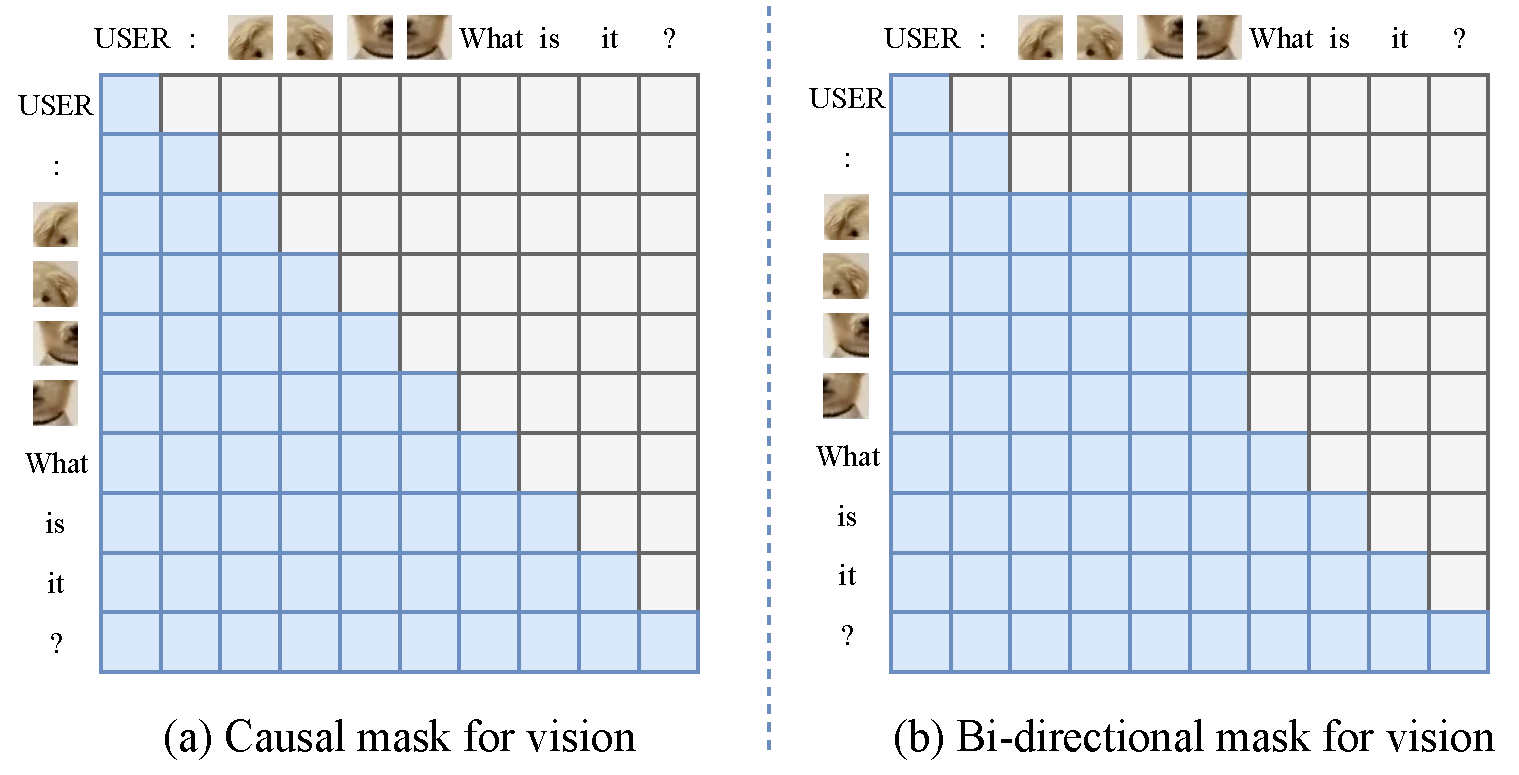
\includegraphics[width=\linewidth]{images/Figure3.pdf}
    \caption{Attention masks for vision: (a) causal attention inherits the autoregressive mask from language modeling, enforcing sequential dependency between image patches; (b) bidirectional attention offers full visibility between all image patches within the same input, enabling global contextual awareness.}
    \label{fig:attention-mask}
\end{figure}

While bi-directional attention masks is common in Transformer architectures in various fields \cite{vit, clip, transfusion}, few studies have explored replacing the causal mask of autoregressive LLMs with a bi-directional mask, especially in the field of MLLMs.

As illustrated in Figure \ref{fig:attention-mask}, we have explored the use of a bi-directional attention mask for vision. Our findings indicate that this attention mask positively impacts the final performance of \model{}, which will be discussed in Section \ref{sec:experiments}. In contrast to prior works \cite{eve, evev2, monointernvl, fuyu}, which have relied on causal masking designed for autoregressive text generation, we demonstrate that adopting bi-directional attention for vision tokens while retaining causal masking for text, not only preserves language capabilities but also enhances visual performance. This aligns with insights from image generation research \cite{transfusion}, highlighting \model{}’s potential as a unified architecture for multimodal generation and understanding tasks.
% \\
% As shown in Figure \ref{fig:attention-mask}, we explored three types of attention masks for vision: (a) causal mask, (b) bidirectional mask, and (c) localized bidirectional mask. While the bidirectional mask demonstrates improved performance, we find that the localized bidirectional mask outperforms it by allowing tokens to focus exclusively on a single image without interference from other text.
% \subsection{Simple Image Patchifier}

% Since we employ \model{} to encode visual information, we can utilize a very lightweight image patchifier. For simplicity, we use the original image patchifier from ViT, along with a single linear layer to align the dimensions, resulting in less than 10M parameters.



\section{Data}
\label{sec:data}
\begin{table}[t]
    \centering
    \renewcommand{\arraystretch}{1.2} % 行间距
    \setlength{\tabcolsep}{2pt} % 减少列间距
    \small
    \begin{tabular}{l|l|c|c}
        \toprule
         Data Format & Dataset & \# Sample & Total \\
         \midrule
        \multirow{2}{*}{Image Caption} & DataComp29M-recap (ours) & 29M & \multirow{2}{*}{30.4M} \\
         & GLDv2-recap (ours) & 1.4M & \\
        \midrule
        \multirow{10}{*}{Text QA} & Infinity-Instruct-3M \cite{infinityinstruct} & 3.5M & \multirow{10}{*}{6.4M} \\
         & SmolTalk \cite{smoltalk} & 1.0M & \\
         & OpenOrca \cite{OpenOrca} & 994.0K & \\
         & MathInstruct \cite{mathinstruct} & 262.0K & \\
         & OrcaMath \cite{orcamath} & 200.0K & \\
         & MagpiePro (L3 ST) \cite{llavaov} & 150.0K & \\
         & WizardCoder \cite{wizardcoder} & 143.0K & \\
         & OpenCodeInterpreter \cite{opencodeinterpreter} & 66.0K & \\
         & MathQA \cite{mathqa} & 29.8K & \\
         & Dolly \cite{dolly} & 11.0K & \\
        \bottomrule
    \end{tabular}
    \caption{Data used in the pre-training stage of \model{}. We use a mixture of both image and text data to alleviate the forgetting issue in training.}
    \label{tab:data}
\end{table}

\subsection{Data collection and preprocessing}
We claim that the primary focus of this work is not on data engineering or filtration; therefore, we adopt a straightforward data collection and processing strategy. Following previous studies \cite{eve, evev2, monointernvl}, our pre-training framework utilized re-captioned data. Given the limited availability of open-source, large-scale re-captioned datasets, we employed Qwen2-VL-72B \cite{qwen2vl} to generate captions for images sampled from DataComp-1B \cite{datacomp}. From this raw dataset, we selected approximately 29 million images with a longer edge exceeding 448 pixels.

We recognize that this dataset lacks specific world knowledge, particularly regarding landmarks, celebrities, and artworks. To address the deficiency in landmark data, we supplemented our dataset with approximately 1.4 million images from the Google Landmarks Dataset v2 (GLDv2) \cite{googlelandmarksdatasetv2}. For other categories, no suitable million-scale datasets were available. Furthermore, due to potential ethical concerns, we chose not to collect such data. Consequently, we acknowledge that our method may underperform in these domains. However, this limitation can be mitigated in future works by integrating relevant datasets. 
% \subsection{Coarse-to-fine data sampling strategy}
% In preliminary experiments, we evaluated caption granularity, specifically standard and detailed captions, to optimize training stability and downstream performance. Our observations indicated that detailed captions introduced instability during early training stages, likely due to the challenges LLMs face in learning fine-grained visual perception, which hindered convergence. In contrast, standard captions improved stability but limited information richness, ultimately capping final performance. To address these trade-offs, we adopted a coarse-to-fine data sampling strategy: during the initial training steps, we exclusively utilized standard captions, and after a predetermined number of steps, we incorporated detailed captions as well. This approach conceptually aligns with the overall training process of modular MLLMs, where the pre-training of the ViT can be viewed as involving relatively coarse supervision, while alignment and fine-tuning \cite{sharegpt4v, llavaov} represent fine-grained supervision.

\subsection{Multimodal data mixture}

While \model{} decouples vision and language parameters, we have observed that extended caption-only training slightly degrades the LLM's instruction-following capability. To preserve this ability, we mixed text instruction data into the training data. As shown in Table \ref{tab:data}, our final mixture contained approximately 30M image-caption pairs and 6.4M text instruction samples. The text data were obtained directly from: Infinity-Instruction \cite{infinityinstruct}, SmolTalk \cite{smoltalk}, Cambrian-1 \cite{cambrian1}, and LLaVA-OneVison \cite{llavaov}.
\section{Experiments}
\label{sec:experiments}
\begin{figure}
    \centering
    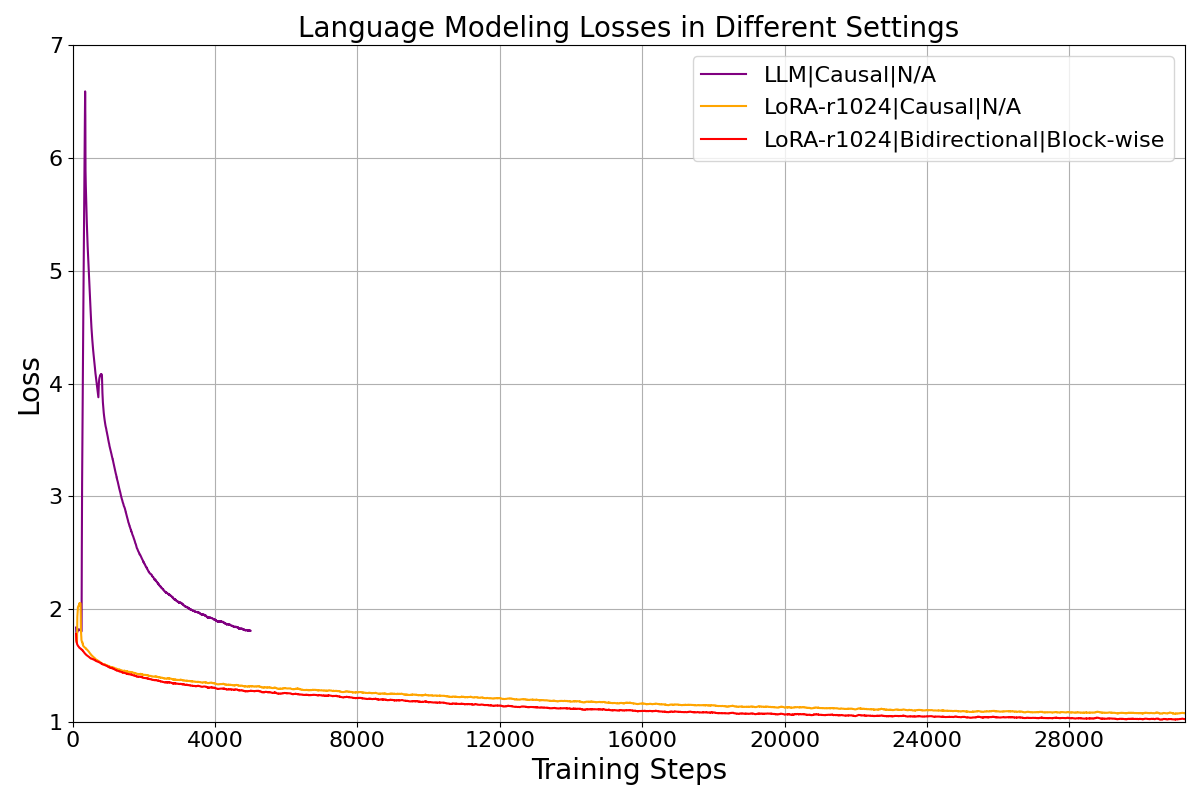
\includegraphics[width=\linewidth]{images/loss_curves_full_llm.png}
    \caption{Language modeling losses in different settings. Training the full LLM with a new modality of data can lead to unrecoverable spike in loss curve, i.e., loss collapse.}
    \label{fig:full_llm}
\end{figure}
\subsection{Implementation details}
\textbf{Training setup.}
Unless otherwise specified, we employed AIMv2-Huge-448p \cite{aimv2} as the default vision encoder and Qwen2.5-7B-Instruct \cite{qwen2.5} as the LLM across all experiments. The pre-training learning rate was fixed at 0.0002 (held constant unless explicitly varied), with 100 warm-up steps and a global batch size maintained at 256. All other hyperparameters and optimizer configurations followed the defaults in \cite{llava1_5}. 

For fine-tuning, all LoRA layers were merged into the LLM, while other components (e.g., distillation modules) were eliminated. The full LLM and 6M-parameter visual embedding layer were trainable. For native-resolution variants (\model{}-AnyRes in Table \ref{tab:ablation}), we retained the pre-trained weights of the fixed-resolution version and adopted native-resolution strategy only during fine-tuning.
\\
\textbf{Benchmarks.} As shown in Table \ref{tab:ablation} and Table \ref{tab:mlm_comparison}, we evaluated the model on several benchmarks: VQAv2: VQAv2 \cite{vqav2}; SQA-I: ScienceQA-Image \cite{scienceqa}; TQA: TextVQA \cite{textvqa}; POPE: POPE \cite{pope}; $\mathrm{MMP_p}$: MME Perception \cite{mme}; $\mathrm{MME_c}$: MME Cognition \cite{mme}; MMB: MMBench \cite{mmbench}; SEED-I: SEED-Image \cite{seed}; MMVet: MMVet \cite{mmvet}; AI2D: AI2D \cite{ai2d}; RQA: Realworld-QA \cite{grok1.5v}; MMMU: MMMU \cite{mmmu}.
% \textbf{Pre-training configurations.} 
% Unless otherwise specified, we employed AIMv2-Huge-448p as our default ViT and Qwen2.5-7B-Instruct as the LLM across all experiments. Detailed hyperparameter settings, including learning rates, batch sizes, and training schedules, were provided in the Appendix.
% \textbf{Visual instruction tuning.} 
% To rigorously evaluate \model{}’s capabilities, we adopted a constrained experimental protocol: using the identical supervised fine-tuning data (LLaVA-665k) and training hyperparameters as LLaVA-1.5 \cite{llava}. This approach enables direct and fair comparison with modular MLLMs and previous monolithic MLLMs \cite{eve, monointernvl} under equivalent data conditions. Our goal is not to outperform via data scaling but to demonstrate that \model{} — despite its monolithic design — achieves performance parity with prevailing modular architectures when given additional pre-training data.
% \textbf{The Setting of ablation studies.} In order to evaluate the impact of key architectural components on visual capability, we curated a subset of 8 million image-text pairs from our DataComp29M-recap dataset.  Text instruction data were excluded from these experiments.
% \textbf{Evaluation Benchmarks.} 
% Our evaluation strategy focuses on two key aspects:
% \begin{itemize}
%     \item \textit{Base Model Capability}: We assess using 10 standard benchmarks: VQAv2, GQA, VizWiz, ScienceQA-Img, TextVQA, POPE, MME, MMBench-EN, Seed-Image, and MM-Vet
%     \item \textit{Ablation Studies}: To accommodate submission limits on VQAv2 and VizWiz, we employ alternative benchmarks for component analysis
% \end{itemize}
% This dual-strategy approach ensures comprehensive validation of \model{}'s core competencies while adhering to platform constraints. All metrics and evaluation protocols align with established practices in multimodal model assessment.
\subsection{Ablation studies}
\begin{figure*}
    \centering
    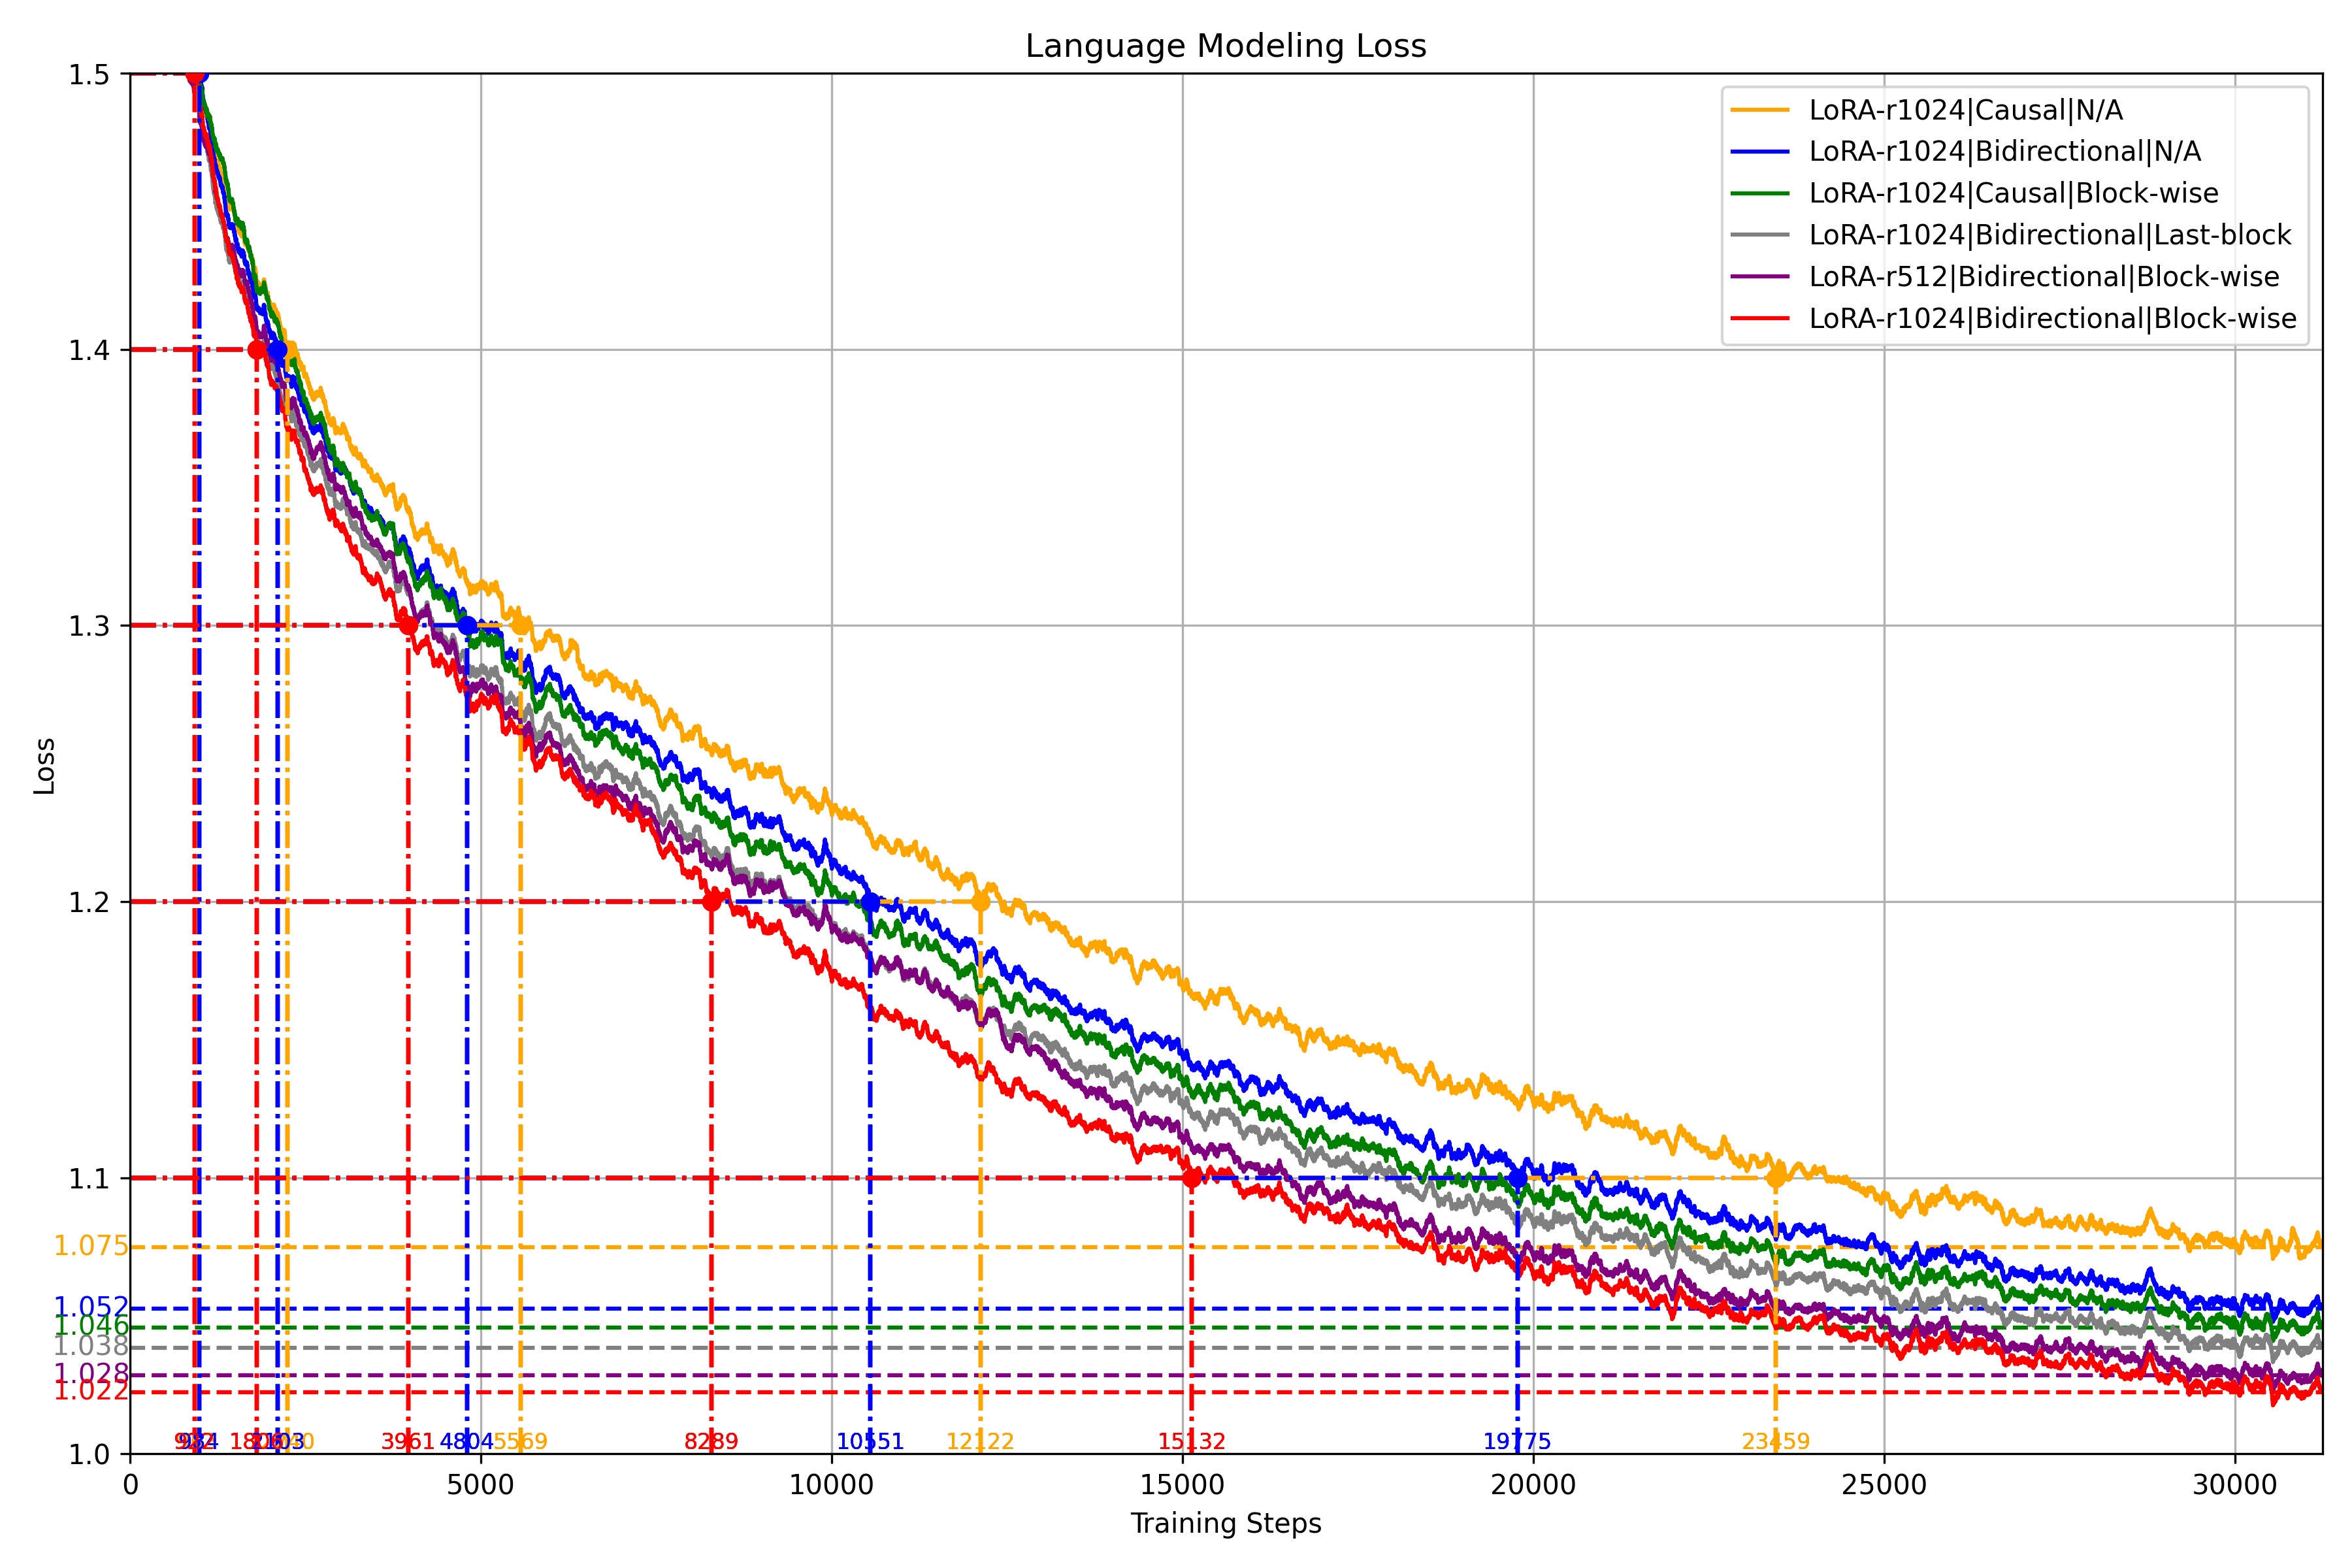
\includegraphics[width=\linewidth]{images/ablation_loss.png}
    \caption{Pre-training loss curves under different configurations. Loss values are smoothed (window=100) for visual clarity. The data sampling order was fixed to ensure fair comparison, as evidenced by the similar trajectories of the loss curves in various settings. LoRA-r1024\textbar Bidirectional\textbar Block-wise refers to the setting: LoRA with rank 1024, bi-directional attention masks for vision, and block-wise distillation. The configuration with the lowest loss was adopted as the default setting in our experiments.}
    \label{fig:ablation_loss}
\end{figure*}
\begin{figure}
    \centering
    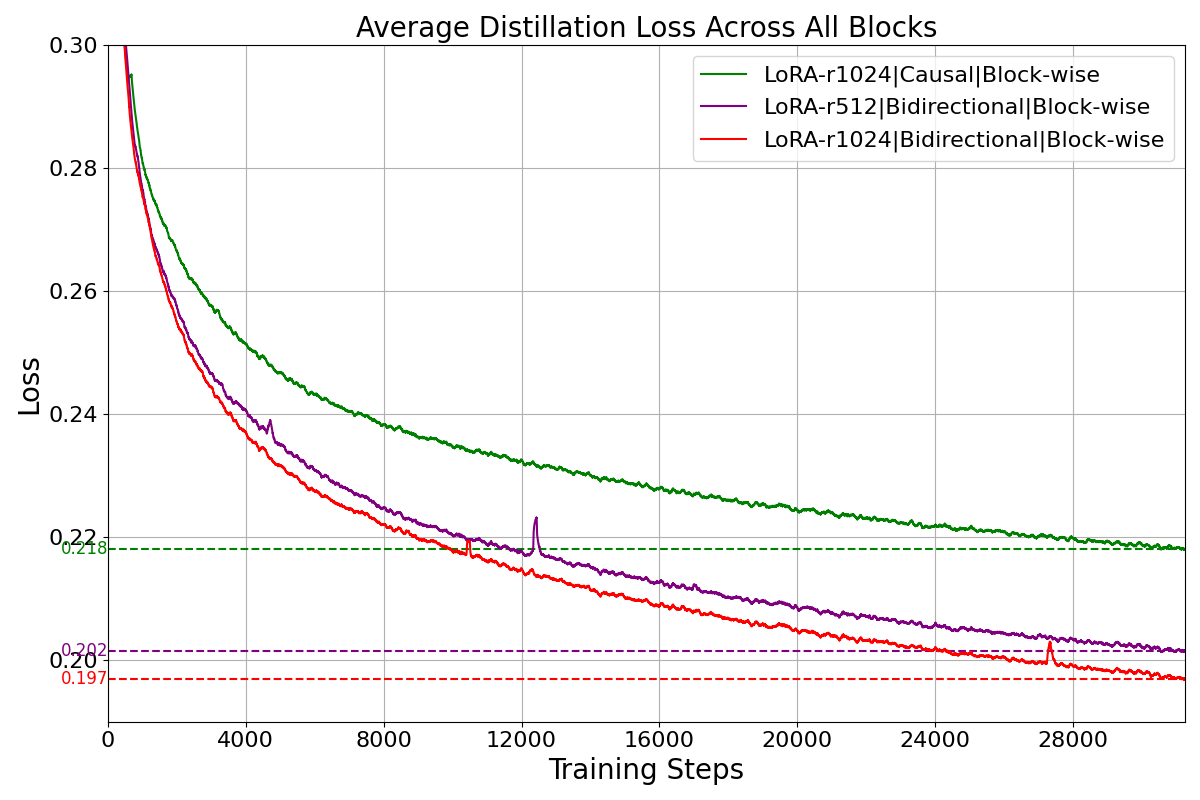
\includegraphics[width=\linewidth]{images/aux_loss_ablation.png}
    \caption{Average distillation loss across all blocks under various settings. Our LoRA-r1024\textbar Bidirectional\textbar Block-wise configuration achieves the lowest average distillation loss across all blocks. This indicates a closer alignment with the ViT’s feature space, confirming that bi-directional attention masks and a larger rank of LoRA layers also enhance visual knowledge transfer.}
    \label{fig:aux_loss}
\end{figure}
% \begin{figure}
%     \centering
%     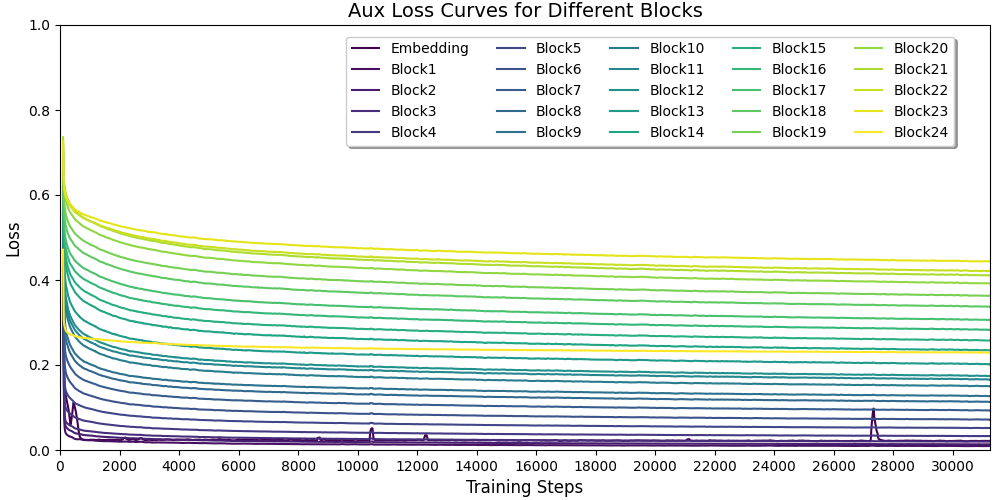
\includegraphics[width=\linewidth]{images/aux_loss.png}
%     \caption{Auxiliary loss for different blocks. loss initially increases with layer depth before declining in later blocks.}
%     \label{fig:aux_loss}
% \end{figure}
\begin{table*}[h]
    \centering
    \renewcommand{\arraystretch}{1.5} % 行间距
    \setlength{\tabcolsep}{3.5pt} % 减少列间距
    \small
    \begin{tabular}{l|c|c|cccccccc|c}
    \toprule
    Vision Params & Visual Attention Mask & Distillation type & TQA & POPE & $\mathrm{MME_p}$ & MMB & SEED-I & MMVet & AI2D & RQA & Avg.\\ 
    \midrule
    % Full LLM (7B) & Causal & N.A. & N.A. & - & - & - & - & - & - & - & - & - \\
    LoRA-r1024 (2B) & Causal & N.A. & 43.7 & 78.6 & 1137.7 & 47.7 & 57.8 & 20.6 & 49.9 & 49.7 & 50.6 \\
    LoRA-r1024 (2B) & Bidirectional & N.A. & 43.6 & 80.9 & 1132.8 & 49.1 & 58.7 & 17.9 & 47.2 & 51.5 & 50.7 \\
    LoRA-r1024 (2B) & Causal & Block-wise & 45.1 & 82.7 & 1172.9 & 52.9 & 63.7 & 20.1 & 50.9 & 51.2 & 53.2 \\
    LoRA-r1024 (2B) & Bidirectional & Last-block & 44.6 & 82.5 & 1197.5 & 51.8 & 63.8 & 17.9 & 49.9 & 52.8 & 52.9 \\
    % LoRA-r1024 (2B) & Bidirectional & Block-wise & AIMv2-Large & - & - & - & - & - & - & - & - & - \\
    LoRA-r512 (1B) & Bidirectional & Block-wise & 47.2 & 83.3 & 1280.5 & 57.6 & 65.3 & 18.5 & 55.9 & 53.1 & 55.6 \\
    % LoRA-r1536 (3B) & Bidirectional & Block-wise & AIMv2-Huge & - & - & - & - & - & - & - & - & - \\
    % LoRA-r1024 (2B) & Bidirectional & Block-wise & Detail & 49.4 & - & - & - & - & - & - & 55.1 & 57.9 \\
    LoRA-r1024 (2B) & Bidirectional & Block-wise & 50.1 & 83.8 & 1224.5 & 53.7 & 65.1 & 22.8 & 52.1 & 55.8 & 55.6 \\
    \bottomrule
    \end{tabular}
    \caption{The performance of various settings on standard benchmarks reveals that lower loss during pre-training correlates with better performance. ``LoRA-r1024 (2B)" indicates that the rank for the LoRA layers is set to 1024, with approximately 2 billion parameters unfrozen for training in total.}
    \label{tab:ablation}
\end{table*}
\begin{figure}
    \centering
    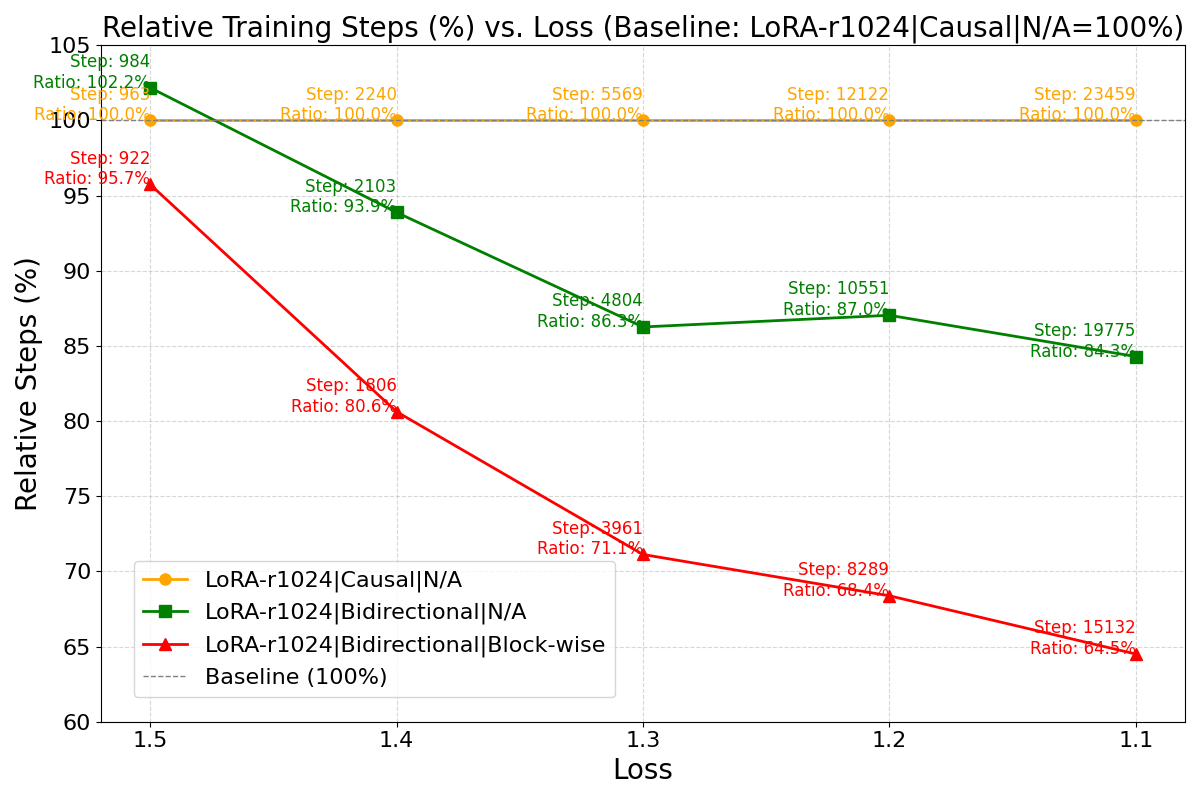
\includegraphics[width=\linewidth]{images/loss_vs_steps.png}
    \caption{Data efficiency analysis. Our experiments demonstrate that combining bi-directional attention masks for vision tokens with block-wise knowledge distillation significantly improves data efficiency compared to the vanilla LoRA configuration. Furthermore, as the target loss decreases (e.g., from 1.5 to 1.1), the required data proportion relative to the baseline diminishes progressively, indicating higher data efficiency.}
    \label{fig:loss_vs_steps}
\end{figure}
Our ablation studies focused on three key components of \model{}: vision as LoRA, block-wise distillation, and bi-directional attention masks for vision. We employed two primary methods to assess performance in various settings: the pre-training loss on an 8M subset of our DataComp29M-recap dataset, as illustrated in Figure \ref{fig:ablation_loss}, and metrics from eight benchmarks, presented in Table \ref{tab:ablation}. Additionally, we visualized the average distillation loss across all blocks, as shown in Figure \ref{fig:aux_loss}.
\\
\textbf{Ablation on vision as LoRA.} Training the full-parameter LLM proved unstable due to modality conflicts (Figure \ref{fig:full_llm}), consistent with findings in \cite{eve}. While reducing the learning rate to a lower value allowed us to observe one successful training case among several attempts, the loss decreased more slowly than that of LoRA-1024. Therefore, we have excluded it from our primary experiments.

Next, we analyzed different LoRA rank configurations in \model{}. Figure \ref{fig:ablation_loss} shows that a rank of 512 resulted in a slightly higher loss (+0.006) compared to rank 1024. This trend continued in the distillation loss (Figure \ref{fig:aux_loss}), where rank 512 showed a modestly higher average block-wise distillation loss (+0.005) compared to rank 1024. Although both configurations ended up with the same average score of 55.6 (Table \ref{tab:ablation}), the consistent loss advantage suggested that higher ranks might have better optimization potential. Furthermore, we experienced training instability with rank 1536, which prompted us to choose rank 1024 as the default configuration.
\\
\textbf{Ablation on bi-directional attention masks.} 
As demonstrated in Figure~\ref{fig:ablation_loss}, under fixed hyperparameters (e.g., LoRA rank and distillation type), the bi-directional attention mask consistently achieved lower training loss compared to causal masking. This empirical advantage was further supported by the reduced average distillation loss across all Transformer blocks, as depicted in Figure~\ref{fig:aux_loss}. Quantitatively, as evidenced in Table~\ref{tab:ablation}, replacing causal masking with bi-directional masks yielded significant performance improvements. For instance, switching from LoRA-r1024\textbar Causal\textbar Block-wise to LoRA-r1024\textbar Bidirectional\textbar Block-wise led to a 2.4-point average score gain, while replacing LoRA-r1024\textbar Causal\textbar N/A with LoRA-r1024\textbar Bidirectional\textbar N/A yielded a gain of 0.1 points.  
\\
\textbf{Block-wise distillation.} As shown in Figure~\ref{fig:ablation_loss} and Table~\ref{tab:ablation}, applying distillation to the final Transformer block alone significantly improved training efficiency. For example, the transition from the configuration LoRA-r1024\textbar{}Bidirectional\textbar{}N/A to LoRA-r1024\textbar{}Bidirectional\textbar{} Last-block yielded a 2.7-point score gain and a 0.016 reduction in loss. Extending distillation to all blocks via block-wise supervision further enhanced performance: compared with LoRA-r1024\textbar{}Bidirectional\textbar{}Last-block, LoRA-r1024\textbar{}Bidirectional\textbar{}Block-wise produced an additional 2.7-point gain and 0.016 loss reduction. These results indicated that the vanilla distillation method, i.e., last-block distillation, could accelerate training, and block-wise distillation could even strengthen this effect.
\\
% \textbf{Data strategy.} We also examined the impact of using detailed versus standard caption data during the early training stage. As shown in Table \ref{tab:ablation}, employing detailed captions for early-stage pre-training was suboptimal compared to using standard captions. This might be due to the rich and intricate visual clues present in the detailed captions, which could be too fine-grained for a model lacking prior visual capabilities to effectively learn from.
% \\
\textbf{Data efficiency analysis.} We measured data efficiency by reporting the relative number of training steps required to reach certain loss thresholds, using vanilla LoRA as the baseline. 

As illustrated in Figure~\ref{fig:loss_vs_steps}, the bi-directional attention variant without distillation (LoRA-r1024\textbar{}Bidirectional\textbar{}N/A) required 102.2\% of the baseline training steps to reach Loss=1.5, whereas adding block-wise distillation (LoRA-r1024\textbar{}Bidirectional\textbar{}Block-wise) reduced this to 95.7\%. The efficiency gap became more pronounced at lower loss: at Loss=1.1, the same configurations needed 84.3\% and 64.5\% of the vanilla LoRA baseline steps, respectively. This demonstrated that our optimal configuration achieved equivalent convergence with 35.5\% fewer training steps than vanilla LoRA.

Furthermore, the ratio of data needed by our best configuration relative to vanilla LoRA decreased over time, implying that comparable performance could be achieved with $N\times$ fewer training data.
\subsection{Standard evaluation}
\begin{table*}[h]
    \centering
    \renewcommand{\arraystretch}{1.5} % 减少行间距
    \setlength{\tabcolsep}{0.6pt} % 减少列间距
    \footnotesize % 或者使用 \footnotesize
    \begin{tabular}{llccccccccccccccccc}
        \toprule
        \multirow{2}{*}{Method} & \multirow{2}{*}{LLM} & \multirow{2}{*}{ViT} & \multicolumn{2}{c}{\# Sample} & \multirow{2}{*}{VQAv2} & \multirow{2}{*}{SQA-I} & \multirow{2}{*}{TQA} & \multirow{2}{*}{POPE} & \multirow{2}{*}{$\mathrm{MME_p}$} & \multirow{2}{*}{$\mathrm{MME_c}$} & \multirow{2}{*}{MMB} & \multirow{2}{*}{SEED-I} & \multirow{2}{*}{MMVet} & \multirow{2}{*}{AI2D} & \multirow{2}{*}{RQA} & \multirow{2}{*}{MMMU}\\
        \cmidrule{4-5}
        & & & Pretrain & Finetune & & & & & & & & & & \\
        \midrule
        % 在这里添加数据行
        \textit{Encoder-based}\\
        \midrule
        \rowcolor{gray!30}  
        BLIP2 \cite{blip2} & Vicuna-13B & EVA-1B & 129M & - & 65.0 & 61 & 42.5 & 85.3 & 1293.8 & - & - & 49.7 & 22.4 & - & - & - \\
        \rowcolor{gray!30}  
        InstructBLIP \cite{instructblip} & Vicuna-7B & EVA-1B & 129M & 1.2M & - & 60.5 & 50.1 & - & - & - & 36 & 58.8 & 26.2 & - & - & - \\
        \rowcolor{gray!30}  
        InstructBLIP \cite{instructblip} & Vicuna-13B & EVA-1B & 129M & 1.2M & - & 63.1 & 50.7 & 78.9 & 1212.8 & - & - & - & 25.6 & - & - & - \\
        LLaVA-1.5 \cite{llava1_5} & Vicuna-7B & CLIP-0.3B & 558K & 665K & 78.5 & 66.8 & 58.2 & 85.9 & 1510.7 & 316.1 & 64.3 & 66.1 & 31.1 & 54.8 & 54.8 & 35.3\\
        % LLaVA-1.5 \cite{aimv2} & Vicuna-7B & AIMv2-0.3B & 8M & 665K & vqav2 & sqa-i & tqa & pope & mmep & mmec & mmb & seed-i & mmvet & ai2d & rqa & mmmu\\
        LLaVA-1.5 \cite{llava1_5} & Qwen2.5-7B & AIMv2-0.6B & 558K & 665K & 82.3 & 77.5 & 59.2 & 85.2 & 1582.3 & 313.0 & 66.3 & 70.6 & 33.7 & 63.7 & 60.0 & 35.3\\
        \midrule
        \textit{Encoder-free}\\
        \midrule
        % \model{} & Qwen2.5-7B & \sout{AIMv2-0.6B} & 8M & 665K & vqav2 & sqa-i & tqa & pope & mmep & mmec & mmb & seed-i & mmvet & ai2d & rqa & mmmu\\
        % \model{} & Qwen2.5-7B & \sout{AIMv2-0.6B} & 8M & 665K & vqav2 & sqa-i & 50.1 & 83.8 & 1224.5 & 274.6 & 53.7 & 65.1 & 22.8 & 52.1 & 55.8 & \\
        \model{} & Qwen2.5-7B & \sout{AIMv2-0.6B} & 30M & 665K & 76.0 & 75.9 & 56.3 & 84.5 & 1363.4 & 311.1 & 64.2 & 67.5 & 33.7 & 65.6 & 57.7 & 32.2\\
       \model{}-AnyRes & Qwen2.5-7B & \sout{AIMv2-0.6B} & 30M & 665K & 76.0 & 72.0 & 58.7 & 85.5 & 1336.1 & 319.3 & 61.3 & 68.9 & 33.7 & 61.1 & 60.1 & 32.0\\
       EVE \cite{eve} & Vicuna-7B & \sout{CLIP-0.3B} & 49M(2) & 665K & 75.4 & 63.0 & 51.9 & 83.6 & 1217.3 & 266 & 49.5 & 61.3 & 25.6 & 48.5 & - & - \\
   \rowcolor{gray!30} 
      EVE-HD \cite{eve} & Vicuna-7B & \sout{CLIP-0.3B} & 49M(2) & 1.8M & 74.2 & 64.9 & 56.8 & 85.0 & 1305.7 & 322 & 52.3 & 64.6 & 25.7 & 61.0 & - & - \\
    \rowcolor{gray!30}  
      EVEv2 \cite{evev2} & Qwen2.5-7B & - & 87M(2) & 22.3M(2) & - & 96.2 & 71.1 & 87.6 & - & - & 66.3 & 71.4 & 45.0 & 74.8 & 62.4 & 39.3 \\
  \rowcolor{gray!30}  
      Mono-InternVL \cite{monointernvl} & Intern1.5-2B & - & 1.2B(2) & 150M(2) & - & 93.6 & 72.6 & - & - & - & 65.5 & 67.4 & 40.1 & 68.6 & - & 33.7 \\
      Mono-InternVL \cite{monointernvl} & Intern1.5-2B & - & 922M & 665K & - & 57 & 49 & - & 1100 & - & - & - & - & 42 & - & - \\
    Mono-InternVL \cite{monointernvl} & Intern1.5-2B & - & 1.2B(2) & 665K & - & 58 & 55 & - & 1110 & - & - & - & - & 46 & - & - \\
        \bottomrule
    \end{tabular}
    \caption{Comparison with previous methods on several benchmarks. Since this paper aims to demonstrate that \model{} is a strong base model, we did not scale the fine-tuning data. Therefore, we did not compare with recent state-of-the-art models that often require additional data engineering or involve proprietary datasets; methods that utilize extra fine-tuning data are grayed out. We classified domain-specific VQA data as fine-tuning data rather than pre-training data for EVEv2 and Mono-InternVL, which differs from their original classification in the respective papers. The notation ``49M(2)" indicates that this method employs a two-stage training process using a total of 49M image-text pairs. The strikethrough notation \sout{ViT} means that ViT is excluded during inference.}
    \label{tab:mlm_comparison}
\end{table*}
To ensure a fair comparison between \model{} and existing methods, we deliberately restricted our experimental design. While prior works (e.g., EVE, EVEv2 \cite{evev2}, and Mono-InternVL \cite{monointernvl}) have leveraged massive in-domain datasets (Table~\ref{tab:mlm_comparison}), such approaches complicated direct comparisons due to proprietary training data. Our goal is not to pursue state-of-the-art performance on benchmarks but to validate a novel MLLM architecture. Thus, we limited fine-tuning to the publicly available LLaVA-665K dataset without additional scaling.

To eliminate the potential advantages provided by LLMs and ViTs, we also trained a LLaVA-1.5 model using Qwen-2.5-7B and AIMv2-0.6B. As shown in Table~\ref{tab:mlm_comparison}, prior encoder-free methods often adopted intricate multi-stage pipelines involving module freezing strategies and proprietary datasets (e.g., 100M–1.2B samples). In contrast, our framework employed a streamlined single-stage training process (pre-training followed by fine-tuning), using about 30M image-text pairs. 
% In contrast to the claims made in EVEv2 \cite{evev2} and Mono-InternVL \cite{monointernvl}, we classified domain-specific VQA data in Table \ref{tab:mlm_comparison} as fine-tuning data rather than pre-training data, aligning with the community's consensus. 

As shown in Table~\ref{tab:mlm_comparison}, \model{} achieved performance comparable to both official and reproduced LLaVA-1.5 baselines on most benchmarks when evaluated under strict LLaVA-1.5 protocols \cite{llava1_5}, i.e., identical prompts/generation parameters. However, \model{} underperformed on MME Perception, a gap we attribute to limited world knowledge in our pre-training data. This was further quantified in Table~\ref{tab:world_knowledge}, where \model{} struggled with tasks demanding intensive world-knowledge: 1) inferring movie details from posters, 2) identifying celebrities, 3) recognizing landmarks, and 4) classifying artworks, as these tasks required external domain knowledge absent in our training datasets.

\begin{table}[]
    \centering
    \renewcommand{\arraystretch}{1.5}
    \small
    \setlength{\tabcolsep}{3pt}
    \begin{tabular}{c|cccc|c}
    \toprule
        Method & Posters & Celebrity & Landmark & Artwork & Total\\
        \midrule
        LLaVA-1.5 & 156.1 & 143.5 & 173.5 & 134.0 & 607.1\\
        \midrule
        VoRA & 117.3 & 111.2 & 139.3 & 105.5 & 473.3\\
        VoRA-AnyRes & 110.2 & 104.7 & 138.0 & 110.8 & 463.7\\
    \bottomrule
    \end{tabular}
    \caption{The performance of VoRA in world knowledge tasks. We acknowledge its deficiency, as expected, due to the lack of relevant in-domain data in our pre-training dataset. This is the primary reason for our lower performance on the MME Perception benchmark.}
    \label{tab:world_knowledge}
\end{table}
\section{Future Work}
\label{sec:conclusion}

We outline several promising directions for future work.

\myparagraph{Faster implementation.}
Our current TTT-MLP kernel is bottlenecked by register spills and suboptimal ordering of asynchronous instructions. Efficiency could probably be further improved by minimizing register pressure and developing a more compiler-aware implementation of asynchronous operations.

\myparagraph{Better integration.} Using bi-direction and learned gates is only one possible strategy for integrating TTT layers into a pre-trained model. Better strategies should further improve generation quality and accelerate fine-tuning. 
Other video generation backbones, such as autoregressive models, might require different integration strategies.

\myparagraph{Longer videos with larger hidden states.} 
Our approach can potentially be extended to generate much longer videos with linear complexity.
The key to achieving that goal, we believe, is to instantiate the hidden states as much larger neural networks than our two-layer MLP.
For example, $f$ itself can be a Transformer.

\vspace{4ex}
\myparagraph{Acknowledgements.} We thank Hyperbolic Labs for compute support, Yuntian Deng for help with running experiments, and Aaryan Singhal, Arjun Vikram, and Ben Spector for help with systems questions.
Yue Zhao would like to thank Philipp Krähenbühl for discussion and feedback.
Yu Sun would like to thank his PhD advisor Alyosha Efros for the insightful advice of looking at the pixels when working on machine learning.

\myparagraph{Note on authorship.} 
Gashon Hussein and Youjin Song joined the team after an initial version of this project was submitted to CVPR, and have made major contributions to the final version.
Because CVPR does not allow us to add authors after submission, their names could not appear on OpenReview and the conference webpage.
However, we all agree that the official author list should include their names, as presented in our released PDFs.
This project would not be possible without their work.
{
    \small
    \bibliographystyle{ieeenat_fullname}
    \bibliography{main}
}


\end{document}
